\section{Background}
The initial research portion of this project focused on several important subjects. In order to gain a complete understanding of the types of sensor technology used in current remote situational awareness products, these devices were investigated first. Research was then performed on prior art in the field of SLAM and depth estimation. Following this research, the Zynq processor and Avnet ZedBoard platform were investigated, and an intended overall system design and sensor suite were defined. 

\subsection{Remote Situational Awareness Products}
Remote situational awareness devices consist of throwable robotic platforms with simple video-streaming capability. One such example is the 110 Firstlook by Endeaver Robotics, seen in Figure \ref{robocop}a, is a throwable, rugged robot that provides real-time situational awareness, and investigates dangerous and hazardous material while keeping its operator out of harm's way. It has four day and night cameras and supports two-way audio. The device is remotely controlled by a tablet operator control unit. With all of this functionality, the 110 Firstlook is currently being used by military personnel \cite{endeavor}.
\par
Similar to the 110 Firstlook, the Bounce Image Explorer is a throwable camera ball that wirelessly transmits a 360$^\circ$ panoramic real-time video stream of its surroundings. The ball receives input from six monochrome WVGA camera modules, and the output video stream can be accessed by tablets and smartphones. This device is still in the trial phase with the United States Law Enforcement \cite{bounceImaging}. The device can be seen in Figure \ref{robocop}b.
\par
A more commercial device is Serveball's Squito\textsuperscript{TM} \cite{serveball}. Squito is a wireless, throwable, 360$^{\circ}$ panoramic camera that implements target detection to stabilize the video feed from its many cameras. It is shown in Figure \ref{squito} below.

\begin{figure}[H]
	\centerline{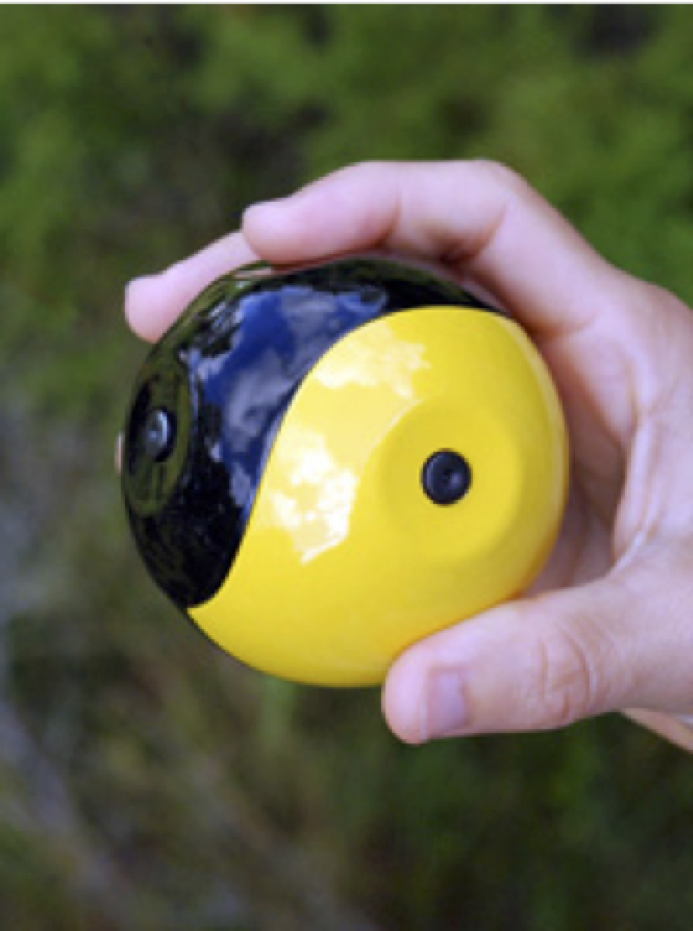
\includegraphics[width=0.3\textwidth]{serveball_squito.png}}
	\caption{Serveball's Squito \cite{serveball}}
	\label{squito}
\end{figure}

Squito utilizes a microprocessor receiving input from cameras, as well as orientation and position sensors, in order to transmit a real-time stabilized video of its adventure. The device is still in the prototype stage and is receiving interest from first responders. The image in Figure \ref{squito_io} shows the input from the Squito's four cameras on the left, and the corresponding stitched output on the right.

\begin{figure}[H]
	\centerline{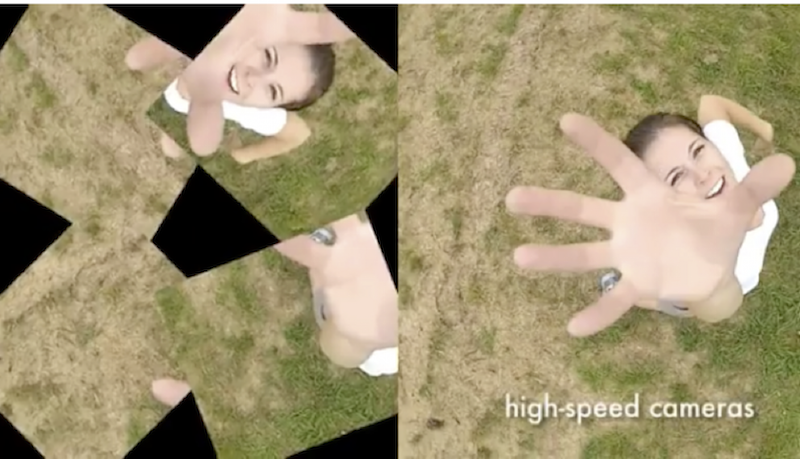
\includegraphics[width=0.6\textwidth]{serveball_io.png}}
	\caption{Serveball's Squito Input and Output \cite{serveball}}
	\label{squito_io}
\end{figure}
\par
After gaining an understanding of the basic imaging functionality contained in current remote situational awareness products, research was performed on improving these systems through the use of Simultaneous Localization and Mapping. 

\subsection{Simultaneous Localization and Mapping}
As mentioned in the previous chapter, Simultaneous Localization and Mapping is the technique of mapping an unknown environment with respect to the device performing said mapping. SLAM is a rapidly expanding field with much potential for improvement, and recent research has focused on making these systems portable. One application of such a system is a proof of concept of camera-based SLAM implementation presented by Andrew Davison of Oxford University in a research paper entitled "Real-Time SLAM with a Single Camera" \cite{davison}. This system is handheld and relies on a computer using a 2.2 GHz Pentium processor connected to a single camera and laser rangefinder. The system requires prior knowledge of the area being analyzed before it can successfully localize and map. It implements edge detection, but is limited to the narrow field of vision of the rangefinder, so it is only able to map an object directly in front of it. This system carries a latency of around 33 milliseconds. An output frame of the device is shown in Figure \ref{rtSLAM}.

\begin{figure}[H]
	\centerline{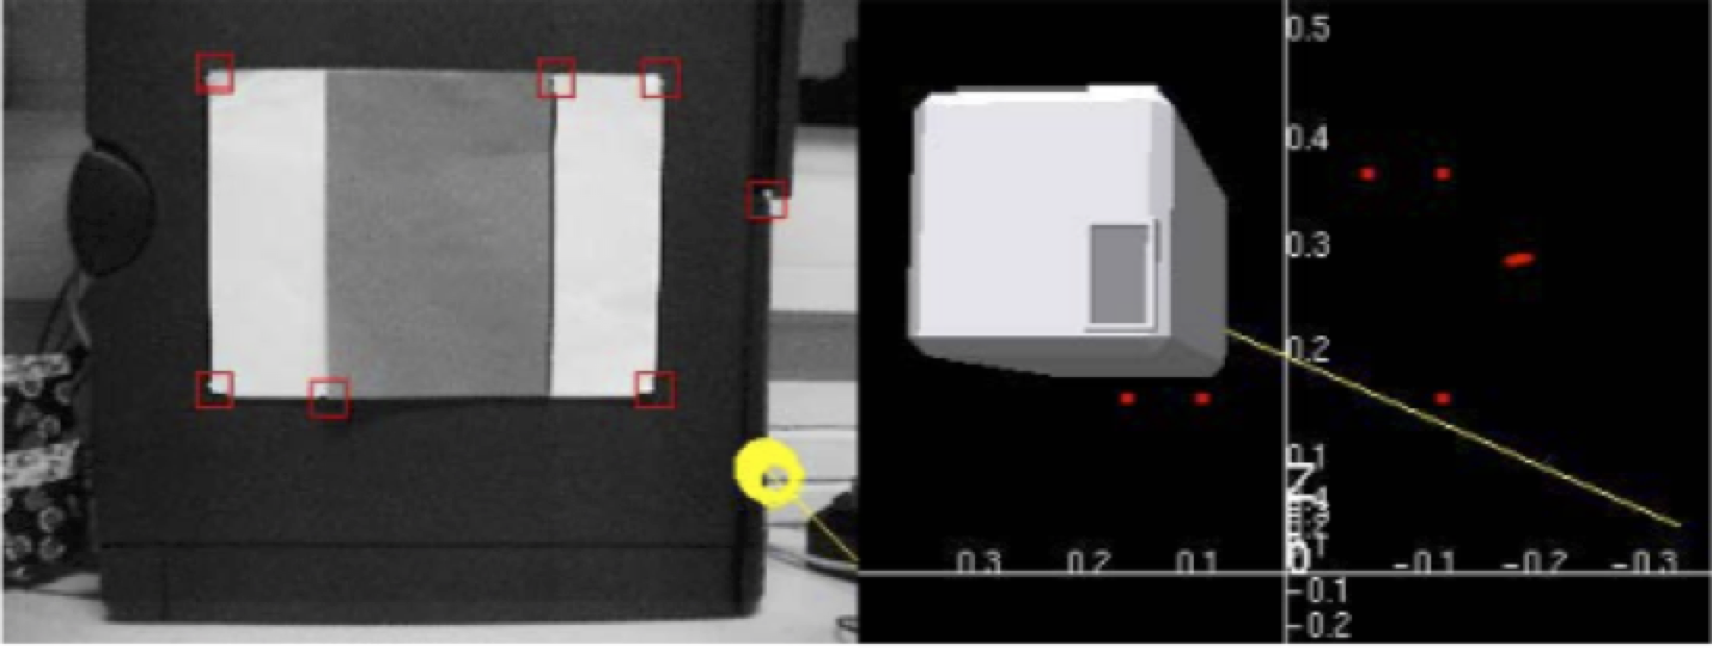
\includegraphics[width=0.8\textwidth]{real_time_SLAM.png}}
	\caption{Real-Time SLAM with a Single Camera \cite{davison}}
	\label{rtSLAM}
\end{figure}

The frame on the left in Figure \ref{rtSLAM} is the video feed with 6 points of a paper target input as prior knowledge, along with successfully marked identifying features (marked as red squares), and another identifying feature that is not marked for measurement (marked by a yellow circle). The frame on the right is a localization graph displaying the positions of all red squares.
\par
By using multiple camera sensors in a sensor suite, it is also possible to determine depth information from corresponding images of an area. This technique is known as stereo imaging, and the process of gathering depth information from a pair of stereo images is known as disparity mapping. University of Bologna researchers Stefano Mattoccia and Matteo Poggi have worked to implement a real-time disparity mapping algorithm on an FPGA, and an example of a stereo image disparity is shown in Figure \ref{disparity_example} below \cite{mattoccia}. Using their stereo vision algorithm, the researchers were able to generate real-time image data showing the relative locations of objects within an image frame using color gradients. Based on this depth information, it is also possible to detect objects located within the field of view of the stereo imaging system, as shown in Figure \ref{disparity_example}. An implementation similar to this is extremely useful in a SLAM-like system, as it allows for the localization of objects and creation of 2D "floorplans" of an area in real-time using only two camera sensors.
\par
\begin{figure}[H]
	\centerline{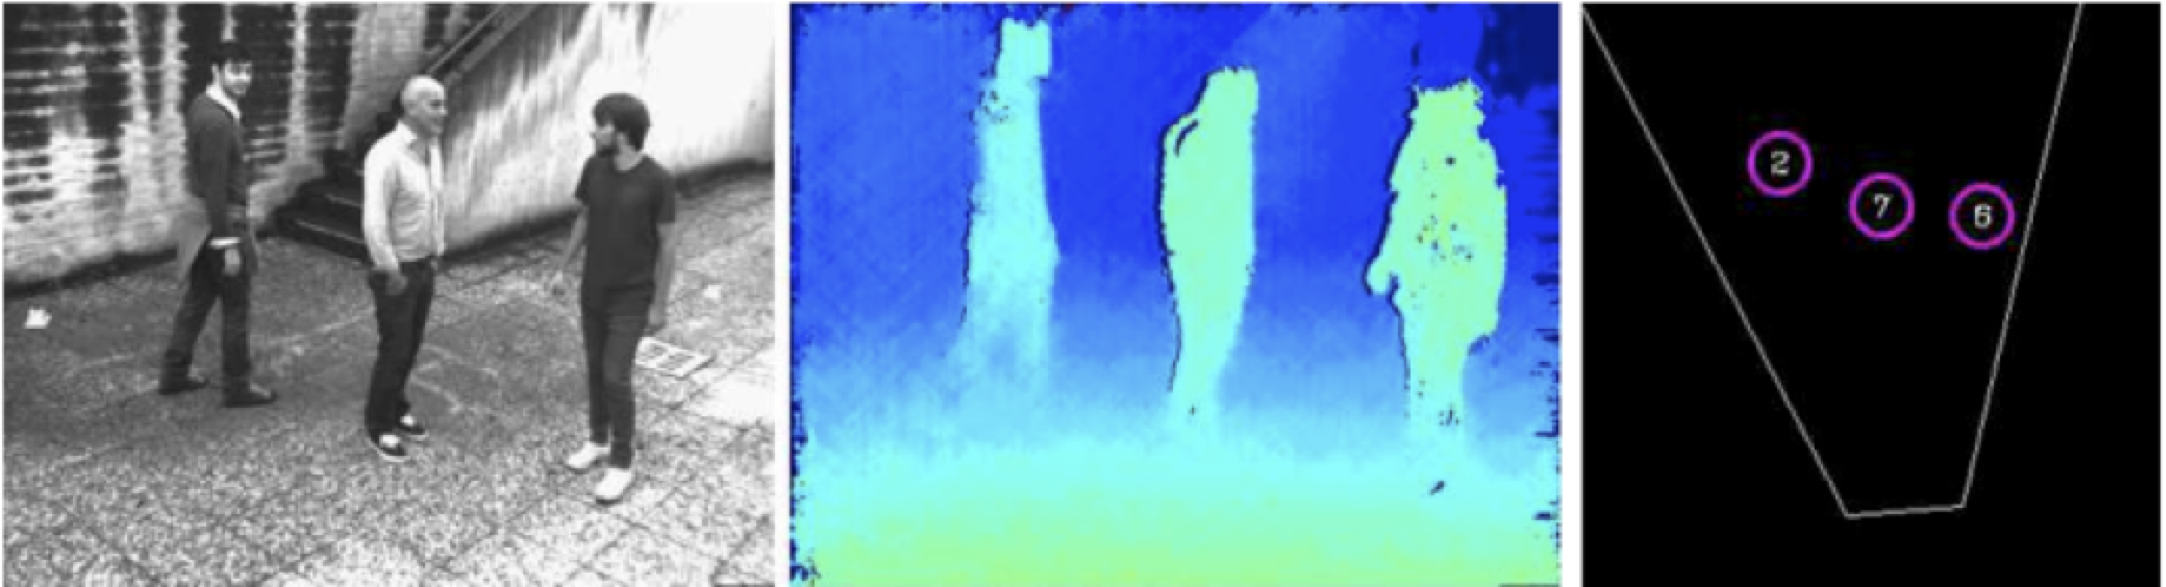
\includegraphics[width=0.9\textwidth]{disparity_example.png}}
	\caption{From Left to Right: Original Image, Disparity Map, Object Detection Results \cite{mattoccia}}
	\label{disparity_example}
\end{figure}
\par
A major concern with real-time image processing, especially in first responder situations, is speed. Because FPGAs have the ability to process data in parallel, they are ideal for this type of application. Using an FPGA for this system will enable all data inputs to be processed at the same time, thereby dramatically increasing throughput speed. 

\subsection{The Zynq Evaluation and Development Board (ZedBoard)}
The ZedBoard is a low-cost development board containing a Xilinx Zynq7000 All-Programmable SoC, and is shown in Figure \ref{zedboard_pic}.

\begin{figure}[H]
	\centerline{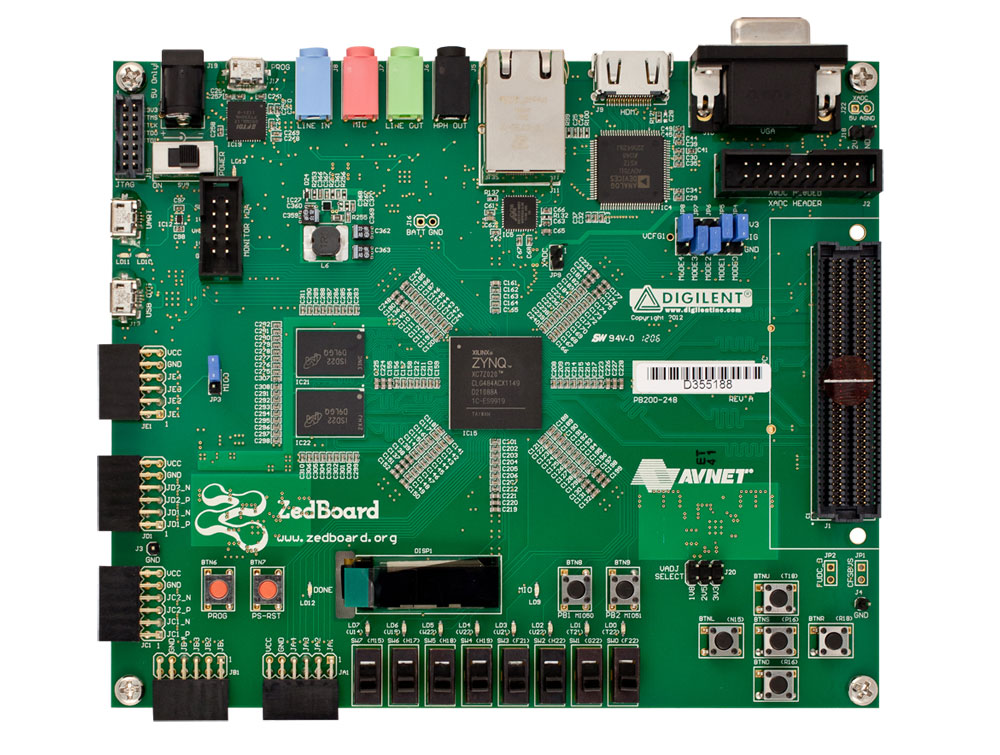
\includegraphics[width=0.75\textwidth]{ZedBoard.jpg}}
	\caption{The Avnet ZedBoard \cite{zedboard_photo}}
	\label{zedboard_pic}
\end{figure}

The Xilinx Zynq-7000 SoC consists of a dual-core ARM Cortex A9 processor coupled with Xilinx Artix-7 FPGA fabric. The ARM Cortex A9 processor uses a dedicated 33.3333 MHz clock source, while the onboard 100 MHz oscillator supplies the PL clock. The Zynq-700 SoC contains 85,000 programmable logic cells with 140 36K block RAM modules. The ZedBoard also features 5 Pmod ports, 8 LEDs, 8 switches, 7 push buttons, a USB UART port, and a VGA port \cite{zedboard_datasheet}. This is shown in the ZedBoard?s block diagram in Figure \ref{zedboardbd}.

\begin{figure}[H]
	\centerline{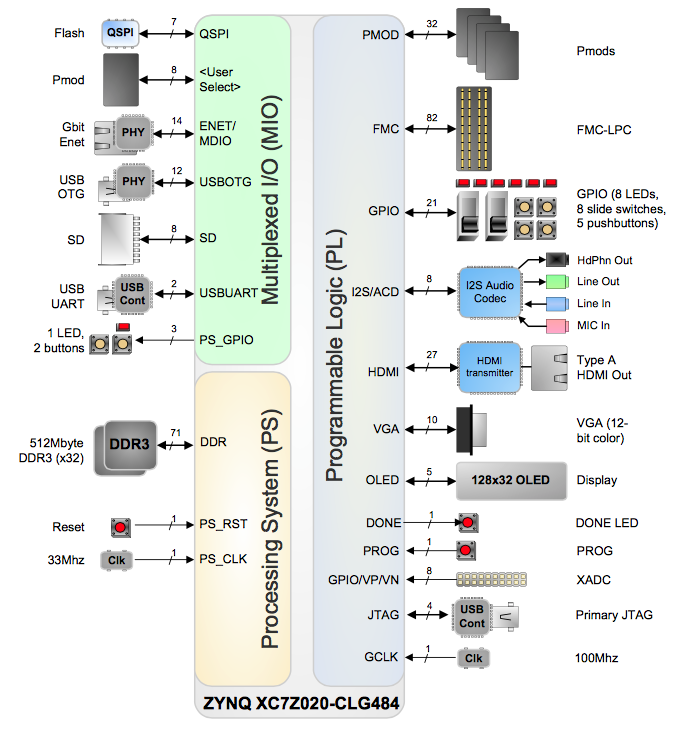
\includegraphics[width=0.75\textwidth]{ZedBoardBD.png}}
	\caption{ZedBoard Block Diagram \cite{zedboard_datasheet}}
	\label{zedboardbd}
\end{figure}
\par
As our research progressed, we believed that we could use a stereo camera pair to gather disparity depth information on an area, and supplement that data with IMU and rangefinder readings in order to produce detailed maps of the sensor suite's surroundings. The envisioned output of this sensor suite was a real-time disparity map of the device?s field of view, as well as a compass-referenced 2D ?floorplan? of the device?s surroundings. An implementation scheme for the creation of this proof of concept sensor suite was then devised, as detailed in the following chapter.